\documentclass{article}

% --- Layout e formattazione generale ---
\usepackage[a4paper, landscape, twocolumn, margin=1.5cm, columnsep=1cm]{geometry}
\usepackage[hidelinks]{hyperref}

% --- Matematica ---
\usepackage{amsthm}
\usepackage{amsmath}
\usepackage{amsfonts}
\usepackage{amssymb}
\usepackage{xcolor}
\numberwithin{equation}{section}
\usepackage{mdframed}
\DeclareMathOperator*{\argmax}{arg\,max}
\DeclareMathOperator*{\argmin}{arg\,min}
\usepackage{cancel}

% --- Teoremi, definizioni e ambienti ---
\renewcommand\qedsymbol{$\blacksquare$}
\newtheorem*{definition}{\color{red}\textbf{Definition}}
\newtheorem*{theorem}{\color{green}\textbf{Theorem}}
\newtheorem*{proposition}{\color{blue}\textbf{Proposition}}
\newmdenv[%
    backgroundcolor=lightgray,
    frametitlebackgroundcolor=gray,
    hidealllines=true,
    frametitlefont=\sffamily\bfseries\color{white},
    frametitle={Example},
]{example}
\newmdenv[%
    backgroundcolor=yellow,
    hidealllines=true
]{recap}

% --- Grafica e disegni ---
\usepackage{graphicx}
\usepackage{wrapfig}
\graphicspath{ {./images/} }


\begin{document}
\pagenumbering{gobble}

\tableofcontents
\clearpage

\pagenumbering{arabic}
\parindent 0pt

\section{Linear Algebra Tools}
This chapter introduces inner product to give geometric meaning to vectors and
vector spaces, enabling calculations of length, distance, and angles.

\begin{definition}[Symmetric Positive Definitive Matrix] 
    A symmetric matrix $A\in \mathbb{R}^{n\times n}$ that satisfies
    \begin{equation}\label{positive_definite_matrix}
        \text{for every nonzero vector }x:x^TAx>0
    \end{equation}    
    is called \textbf{positive definite}. If only $\geq$ holds in
    \ref{positive_definite_matrix}, then $A$ is called \textbf{positive
    semidefinite}.
\end{definition}
These properties helps in identifying positive definite matrices without
having to check the definition explicitly:
\begin{enumerate}
    \item The null space of $A$ contains only the null vector; 
    \item The diagonal elements $a_{ii}$ of $A$ are positive; 
    \item The eigenvalues of $A$ are real and positive.
\end{enumerate}
\subsection{Angles and Orthogonality}
The angle $\omega$ between vectors $x$ and $y$ is computed as:
$$\cos\omega=\frac{\langle x,y\rangle}{\lVert x\rVert_2 \lVert y\rVert_2}$$ 
Here, $\langle x,y\rangle$ denotes the inner product between $x$ and $y$.

This angle indicated the vectors' similarity in orientation. 
\begin{definition}[Orthogonal vectors]
    Two vectors are orthogonal if $\langle x,y \rangle=0$. If additionally
    $\lVert x\rVert=1=\lVert y\rVert$, then $x$ and $y$ are orthonormal.
\end{definition}
\begin{definition}[Orthogonal matrix]
    A square matrix is an orthogonal matrix if and only if \underline{its columns are
    orthonormal} so that 
    $$AA^T=I=A^TA$$
    which implies that 
    $$A^{-1}=A^T$$
\end{definition}
The length of a vector $x$ is not changed when transforming it using an
orthogonal matrix $A$.
$$\lVert Ax\rVert_2^2=\lVert x\rVert_2^2$$
Moreover, the angle between any two vectors $x,y$ is also unchanged when
transforming both of them using an orthogonal matrix $A$.
\begin{definition}[Orthonormal Basis]
    In an $n$-dimensional vector space $V$ with a basis set
    $\{b_1,\ldots,b_n\}$, if all the basis vectors are orthogonal to each
    other, the basis is called as an \textbf{orthogonal basis}.
    Additionally, if the length of each basis vector is 1, the basis is
    referred to as an \textbf{orthonormal basis}.
\end{definition}
We can also have vector spaces that are orthogonal to each other. Given a
vector space $V$ of dimension $D$, let's  consider a subspace $U$ of dimension
$M$ such that $U\subseteq V$. Then its \textbf{orthogonal complement}
$U^{\perp}$ is a $D-M$ dimensional subspace $V$ and contains all vectors in
$V$ that are orthogonal to every vector in $U$.
\begin{center}
    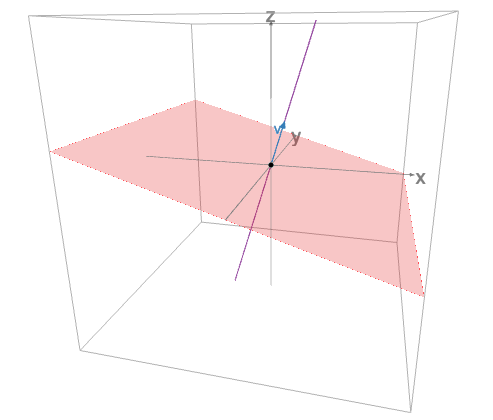
\includegraphics[width=0.6\linewidth]{images/orthogonal_complement}
\end{center}
\subsubsection{Orthogonal Projections}
Projections are key linear transformations in machine learning and are
particularly useful for handling high-dimensional data. Often, only a few
dimensions in such data are essential for capturing the most relevant
information. By projecting the original high-dimensional data onto a lower
dimensional feature space, we can work more efficiently to learn about the
dataset and extract significant patterns.
\begin{definition}[Projection]
    Let $V$ be a vector space and $U\subseteq V$ a subspace of $V$. A linear
    mapping $\pi:V\to U$ is called \textbf{projection} if it satisfies
    $\pi^2=\pi\circ\pi=\pi$.
\end{definition}
Given that linear mappings can be represented by transformation matrices, the
above definition extends naturally to \textit{projection matrices} $P_{\pi}$.
These matrices exhibit the property that $P_{\pi}^2=P_{\pi}$.

The projection $\pi_U(x)$ of a vector $x\in \mathbb{R}^n$ onto a subspace $U$
is the closest point necessarily in $U$ to $x$.
\cleardoublepage
\section{Matrix Decompositions}
\subsection{Eigenvalues and Eigenvectors}
Eigenanalysis helps us understand linear transformations represented by a
matrix $A$. Eigenvectors $x$ are special vectors that only get scaled, not
rotated, when multiplied by $A$. The scaling factor is the eigenvalue
$\lambda$, which indicated how much $x$ is stretched or shrunk. $\lambda$ can
also be zero.
\begin{definition}[Eigenvalue and Eigenvector]
    Let $A\in \mathbb{R}^{n\times n}$ be a square matrix. Then $\lambda\in
    \mathbb{R}$ is an \textbf{eigenvalue} of $A$ and nonzero vector $x$ is the
    corresponding \textbf{eigenvector} of $A$ if 
    \begin{equation}\label{eq:eigenvalue_equation}
        Ax=\lambda x
    \end{equation}
    We call \ref{eq:eigenvalue_equation} the \textbf{eigenvalue equation}.
\end{definition}
The following statements are equivalent:
\begin{itemize}
    \item $\lambda$ is an eigenvalue of $A\in \mathbb{R}^{n\times n}$.
    \item A nonzero vector $x$ exists such that $Ax=\lambda x$ or,
        equivalently, $(A-\lambda I_n)x=0$ for $x\neq 0$.
    \item Then $A-\lambda I$ is a \textbf{singular
        matrix} and its determinant is \textbf{zero}.
\end{itemize}
Each eigenvector $x$ has one unique eigenvalue $\lambda$, but each $\lambda$
can have multiple eigenvectors.
\begin{definition}[Eigenspace and Eigenspectrum]
    For $A\in \mathbb{R}^{n\times n}$, the set of all eigenvectors of $A$
    associated with an eigenvalue $\lambda$ spans a subspace of
    $\mathbb{R}^n$, which is called the \textbf{eigenspace} of $A$ with
    respect to $\lambda$ and is denoted by $E_{\lambda}$. The set of all
    eigenvalues of $A$ is called the \textbf{eigenspectrum} of $A$.
\end{definition}
\begin{definition}
    Let $\lambda_i$ be an eigenvalue of a square matrix $A$. Then the
    \textbf{geometric multiplicity} of $\lambda_i$ is the number of linearly
    independent eigenvectors associated with $\lambda_{i}$. In other words, it
    is the dimensionality of the eigenspace spanned by the eigenvectors
    associated with $\lambda_i$.
\end{definition}
\begin{theorem}
    The eigenvectors $x_1,\ldots,x_n$ of a matrix $A\in \mathbb{R}^{n\times
    n}$ with $n$ distinct eigenvalues $\lambda_1,\ldots,\lambda_n$ are
    linearly independent.
\end{theorem}
This theorem states that eigenvectors of a matrix with $n$ distinct eigenvalues
form a basis of $\mathbb{R}^n$.
\cleardoublepage
\section{Vector calculus}
Firstly, we'll explore partial derivatives and gradients, focusing on functions that take a vector as input and produce a
single real number as output. These functions are formally represented as
$f:\mathbb{R}^n\to \mathbb{R}$.

Subsequently, we will extend these ideas to functions that not only take a
vector as input but also produce a vector as output. These functions can be
written as $f:\mathbb{R}^n\to \mathbb{R}^m$.

\subsection{Gradients of Real-Valued Functions}
When we deal with a function that depends on multiple variables, such as 
$f(x)=f(x_1,x_2)$, we use the \textbf{gradient} to represent its derivative.
The gradient is a vector composed of \textbf{partial derivates} of the
function. To compute each partial derivates, we differentiate the function
with respect to one variable while keeping all other variables constant.
\begin{equation}\label{eq:gradient_real_valued_functions}
   \nabla_x f=\begin{bmatrix}
       \frac{\partial{f}}{\partial{x_1}} &
       \frac{\partial{f}}{\partial{x_2}} & \cdots &
       \frac{\partial{f}}{\partial{x_n}}
    \end{bmatrix}\in \mathbb{R}^{1\times n} 
\end{equation}
where $n$ is the number of variables.
\paragraph{Basic Rules of Partial Differentiation}
\begin{itemize}
    \item[] Product rule:
        $$\frac{\partial}{\partial{x}}(f(x)g(x))=\frac{\partial{f}}{\partial{x}}g(x)+f(x)\frac{\partial{g}}{\partial{x}}$$
    \item[] Sum rule:
        $$\frac{\partial}{\partial{x}}(f(x)+g(x))=\frac{\partial{f}}{\partial{x}}+\frac{\partial{g}}{\partial{x}}$$
    \item [] Chain rule:
        $$\frac{\partial}{\partial{x}}(g\circ
        f)(x)=\frac{\partial}{\partial{x}}\left(g(f(x))\right)=\frac{\partial{g}}{\partial{f}}\frac{\partial{f}}{\partial{x}}$$
\end{itemize}

In the context of the chain rule, consider $f$ as implicitly a composition
$f\circ g$.

If a function $f(x_1,x_2)$ is a function of $x_1$ and $x_2$, where
$x_1(t)$ and $x_2(t)$ are themselves functions of a single variable $t$, the
chain rule yields the partial derivates
$$\frac{\text{d}f}{\text{d}t}=\begin{bmatrix}
    \frac{\partial{f}}{\partial{x_1}} & \frac{\partial{f}}{\partial{x_2}}
    \end{bmatrix}\begin{bmatrix}
    \frac{\partial{x_1(t)}}{\partial{t}} \\ 
    \frac{\partial{x_2(t)}}{\partial{t}}
\end{bmatrix}=\frac{\partial{f}}{\partial{x_1}}\frac{\partial{x_1}}{\partial{t}}+\frac{\partial{t}}{\partial{x_2}}\frac{\partial{x_2}}{\partial{t}}$$
\newpage
\begin{example}
    Consider $f(x_1,x_2)=x_1^2+2x_2$, where $x_1=\sin t$ and $x_2=\cos t$,
    then
    $$\text{with}\quad\frac{\partial{f}}{\partial{x_1}}=2x_1,\quad \frac{\partial{f}}{\partial{x_2}}=2$$
    $$\begin{aligned}
        \frac{\text{d}f}{\text{d}t}&=2\sin t \frac{\partial{\sin t}}{\partial{t}}+2 \frac{\partial{\cos
        t}}{\partial t}\\
            &=2\sin t\cos t-2\sin t
    \end{aligned}$$
\end{example}
If a function $f(x_1,x_2)$ is a function of $x_1$ and $x_2$, where $x_1(s,t)$
and $x_2(s,t)$ are themselves functions of two variables $s$ and $t$, the
chain rule yields the partial derivates
$$
\frac{\text{d}f}{\text{d}(s,t)}=\begin{bmatrix}
    \frac{\partial{f}}{\partial{s}} & \frac{\partial{f}}{\partial{t}}
\end{bmatrix} 
$$
where 
$$
\begin{aligned}
    \frac{\partial{f}}{\partial{s}}&=\frac{\partial{f}}{\partial{x_1}}\frac{\partial{x_1}}{\partial{{\color{red}s}}}+\frac{\partial{f}}{\partial{x_2}}\frac{\partial{x_2}}{\partial{{\color{red}s}}}\\
    \frac{\partial{f}}{\partial{t}}&=\frac{\partial{f}}{\partial{x_1}}\frac{\partial{x_1}}{\partial{{\color{blue}t}}}+\frac{\partial{f}}{\partial{x_2}}\frac{\partial{x_2}}{\partial{{\color{blue}t}}}\\
\end{aligned}
$$
Another way to obtain these two partial derivatives is to represent the
previous formula as a row vector containing the partial derivatives of $f$
with respect to $x_1$ and $x_2$. This row vector is then multiplied by a
matrix composed of the partial derivatives of $x_1$ and $x_2$ with respect to
$s$ and $t$. When you perform this multiplication, you get the exact same
result as above.
$$
\begin{bmatrix}
    \frac{\partial{f}}{\partial{s}} & \frac{\partial{f}}{\partial{t}}
\end{bmatrix}=\begin{bmatrix}
    \frac{\partial{f}}{\color{red}\partial{x_1}} &
    \frac{\partial{f}}{\color{blue}\partial{x_2}}
\end{bmatrix}\begin{bmatrix}
    {\color{red}\frac{\partial{x_1}}{\partial{s}}} &
    {\color{red}\frac{\partial{x_1}}{\partial{t}}} \\ 
    {\color{blue}\frac{\partial{x_2}}{\partial{s}}} &
    {\color{blue}\frac{\partial{x_2}}{\partial{t}}}
\end{bmatrix}$$
\newpage
\begin{example}
    Given the following functions:\\
    $g:\mathbb{R}^2\to \mathbb{R}^2\quad g(s,t)=(\sin(t)s, \cos(s)t)$\\ 
    $f:\mathbb{R}^2\to \mathbb{R}\quad f(x_1,x_2)=x_1^2+2x_2$\\ 
    $f\circ g: \mathbb{R}^2\to \mathbb{R}$\\
    Compute $\nabla_{(s,t)}(f\circ g)$ and evaluate $\nabla_{(s,t)}(f\circ g)(0,0)$.
    $$
    \begin{aligned}
        &=\begin{bmatrix}
            2s\sin(t) & 2
        \end{bmatrix}
        \begin{bmatrix}
            \sin(t) & s\cos(t)\\ 
            -t\sin(s) & \cos(s)
        \end{bmatrix} \\ 
        &=\begin{bmatrix}
            2s\sin^2(t)-2t\sin(s) \\ 
            2s^2\sin(t)\cos(t)+2\cos{t}
        \end{bmatrix}=(0,2)
    \end{aligned}
    $$
\end{example}
\subsection{Gradients of Vector-Valued Functions}
We can express a vector-valued function $f:\mathbb{R}^n\to \mathbb{R}^m$ as a
column vector of $m$ real-valued functions $f_i:\mathbb{R}^n\to \mathbb{R}$.
Given an input vector $x=\begin{bmatrix} x_1,\ldots,x_n \end{bmatrix}^T\in
\mathbb{R}^n$, the output is defined as: 
$$
f(x)=\begin{bmatrix} f_1(x)\\
\vdots \\ f_m(x) \end{bmatrix}\in \mathbb{R}^m
$$
\begin{definition}[Jacobian]
    By contrast, in Equation \ref{eq:gradient_real_valued_functions}, each partial
    derivative $\frac{\partial f}{\partial x_i}$ is a column vector.
    $$
    \begin{aligned}
        J=\nabla_x f&=\begin{bmatrix}
            \frac{\partial{f}}{\partial{x_1}} & \cdots &
            \frac{\partial{f}}{\partial{x_n}}
        \end{bmatrix} \\ 
                  &=\begin{bmatrix}
                      \frac{\partial{f_1}}{\partial{x_1}} & \cdots &
                      \frac{\partial{f_1}}{\partial{x_n}} \\ 
                      \vdots & & \vdots \\ 
                      \frac{\partial{f_m}}{\partial{x_1}} & \cdots &
                      \frac{\partial{f_m}}{\partial{x_n}} \\ 
                  \end{bmatrix}\\
            J(i,j)&=\frac{\partial f_i}{\partial{x_j}}
    \end{aligned}
    $$
    The collection of all first-order partial derivatives of a vector-valued
    function $f:\mathbb{R}^n\to \mathbb{R}^m$ is called the \textbf{Jacobian}.
    The Jacobian $J$ is an $m\times n$ matrix.
\end{definition}
\newpage
\begin{example}
    $f:\mathbb{R}^2\to \mathbb{R}^3,\quad f:(x_1,x_2)=\begin{pmatrix}
        x_1+x_2 \\ 
        2x_1^2-x_2 \\ 
        -x_1x_2
    \end{pmatrix}$\\ 
    $J(f):\mathbb{R}^2\to \mathbb{R}^{3\times 2},\quad J(i,j)=\begin{bmatrix}
        1 & 1 \\ 
        4x_1 & -1 \\ 
        -x_2 & -x_1 
    \end{bmatrix},\quad
    J(1,1)=\begin{bmatrix}
        1 & 1 \\ 
        4 & -1 \\ 
        -1 & -1
    \end{bmatrix}$
\end{example}
\begin{example}
   Let us consider the linear model 
   $$y=\Phi\theta$$
   where $\theta\in \mathbb{R}^D$ is a parameter vector, $\Phi\in
   \mathbb{R}^{N\times D}$ are input features, and $y\in \mathbb{R}^N$ are the
   corresponding observations. We define the functions 
   $$\begin{aligned}
       e:\mathbb{R}^D\to \mathbb{R}^N,\quad e(\theta)&=y-\Phi\theta \\
       L:\mathbb{R}^N\to \mathbb{R},\quad L(e)&=\lVert e\rVert_2^2, \quad
       L(\theta)= \lVert y-\Phi\theta\rVert_2^2
   \end{aligned}$$
   This is called a \textbf{least-squares loss} function.\\ We want to find
   $\frac{\partial{L}}{\partial{\theta}}$, which is derivative of the loss
   function with respect to the parameters $\theta$. This will allow us to
   find the optimal $\theta$ that minimizes the loss function $L(\theta)$.

   The chain rule allows us to compute the gradient as 
   $$\frac{\partial{L}}{\partial{e}}={\color{red}\frac{\partial{L}}{\partial{e}}}{\color{blue}\frac{\partial{e}}{\partial{\theta}}}$$
   We know that $\lVert e\rVert_2^2=e^Te$ and so 
   $${\color{red}\frac{\partial{L}}{\partial{e}}=2e^T}\in \mathbb{R}^{1\times
   N}$$
   Furthermore, we obtain 
   $${\color{blue}\frac{\partial{e}}{\partial{\theta}}=-\Phi}\in
   \mathbb{R}^{N\times D}$$
   such that our desired derivative is
   $$
   \nabla{L}_{\theta}=-2e^T\Phi=-2\underbrace{\color{red}(y^T-\theta^T\Phi^T)}_{1\times
   N}\underbrace{\color{blue}\Phi}_{N\times D}\in \mathbb{R}^{1\times D}\\ 
   $$
\end{example}
\subsection{Backpropagation and Automatic Differentiation}
In machine learning, finding optimal model parameters often involves
performing gradient descent. This requires computing the gradient of a
learning objective with respect to the model's parameters. Calculating the
gradient explicitly can be impractical due to the complexity and length of the
resulting derivative equations. To address this, the \textbf{backpropagation} algorithm
was introduced in 1962 as an efficient way to compute these gradients,
particularly for neural networks.



In neural networks, the output $y$ is computed through a multi-layered
function composition $y=(f_K\circ f_{K-1}\circ \cdots f_1)(x)$. Here, $x$ are
the inputs (e.g., images), $y$ are the observations (e.g., class labels).
Each functions $f_i,i=1,\ldots,K$, has its own parameters.
Specifically, in the $i^{th}$ layer, the function is given
$f_i(x_{i-1})=\sigma(A_{i-1}+b_{i-1})$, where $x_{i-1}$ is
the output from layer $i-1$ and $\sigma$ is an activation function. 
\begin{center}
    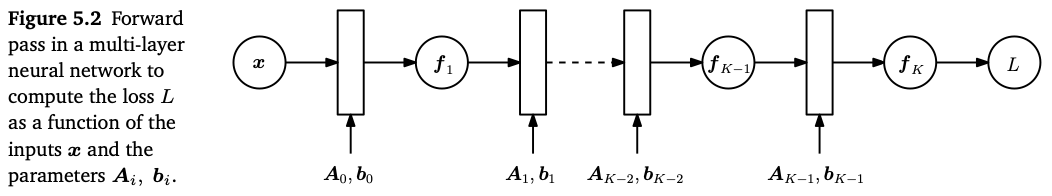
\includegraphics[width=\linewidth]{nn_forward_pass}
\end{center}
In order to train a neural network, we aim to minimize a loss function $L$
with respect to all parameters $A_j,b_j$ for $j=0,\ldots,K-1$.
Specifically, we're interested in optimizing these parameters to minimize the
squared loss given by
$$L(\theta)=\lVert y-f_K(\theta,x)\rVert^2$$
where $\theta=\{A_0, b_0, \ldots,A_{K-1},b_{K-1}\}$.

To minimize $L(\theta)$ we need to compute its gradients of $L$ to the
parameter set $\theta$. This involes calculating the partial derivatives of
$L$ with respect to the parameters $\theta_j=\left\{A_j,b_j\right\}$ for each
layer $j=0,\ldots,K-1$. The chain rule allows us to determine the partial
derivatives as
$$\begin{aligned}
    \frac{\partial{L}}{\partial{\theta_{K-1}}}&=\frac{\partial{L}}{\partial{f_K}}{\color{blue}\frac{\partial{f_K}}{\partial{\theta_{K-1}}}}
    \\
    \frac{\partial{L}}{\partial{\theta_{K-2}}}&=\frac{\partial{L}}{\partial{f_K}}\boxed{{\color{red}\frac{\partial{f_K}}{\partial{f_{K-1}}}}{\color{blue}\frac{\partial{f_{K-1}}}{\partial{\theta_{K-2}}}}}
    \\
    \frac{\partial{L}}{\partial{\theta_{K-3}}}&=\frac{\partial{L}}{\partial{f_K}}{\color{red}\frac{\partial{f_K}}{\partial{f_{K-1}}}}\boxed{{\color{red}\frac{\partial{f_{K-1}}}{\partial{f_{K-2}}}}{\color{blue}\frac{\partial{f_{K-2}}}{\partial{\theta_{K-3}}}}}
    \\
    \frac{\partial{L}}{\partial{\theta_{i}}}&=\frac{\partial{L}}{\partial{f_K}}{\color{red}\frac{\partial{f_K}}{\partial{f_{K-1}}}\cdots}\boxed{{\color{red}\frac{\partial{f_{i+2}}}{\partial{f_{i+1}}}}{\color{blue}\frac{\partial{f_{i+1}}}{\partial{\theta_{i}}}}}
\end{aligned}$$
The {\color{red}red} terms are partial derivatives of the output of a layer
with respect to its inputs, whereas the {\color{blue}blue} terms are partial
derivatives of the output of a layer with respect to its parameters. 

The key insight of backpropagation is to reuse previously computed derivatives
to avoid redundant calculations. When we've computed the partial derivatives
$\frac{\partial{L}}{\partial{\theta_{i+1}}}$, we can reuse them to efficiently
calculate the partial derivatives
$\frac{\partial{L}}{\partial{\theta}_{i}}$.

It turns out that backpropagation is a special case of a set of techniques
known as \textbf{automatic differentiation}. Automatic differentiation
numerically evaluate the exact (up to machine precision) gradient of a function by working with
intermediate variables and applying the chain rule.

\begin{center}
    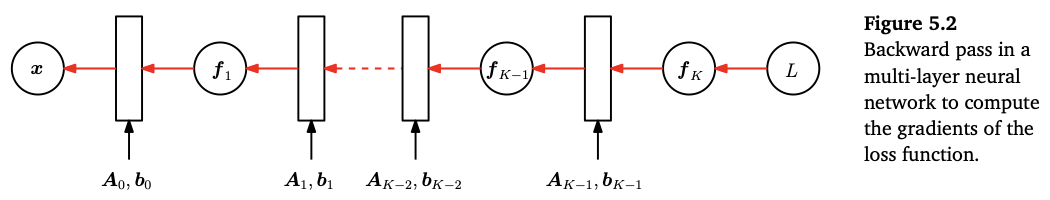
\includegraphics[width=\linewidth]{nn_backward_pass}
\end{center}
\begin{example}
    Consider the real-valued function 
    $$f(x)=\sqrt{x^2+\exp(x^2)}+\cos(x^2+\exp(x^2))$$
    Another way to attach this would be to just define some \textit{intermediate
    variables}. Say 
    $$
    \begin{aligned}
        a=x^2\\
        b=\exp(a)\\ 
        c=a+b\\ 
        d=\sqrt{c}\\ 
        e=\cos(c)\\ 
        f=d+e
    \end{aligned}
    $$
    The set of equations that include intermediate variables can be thought of
    as a computational graph 
    \begin{center}
        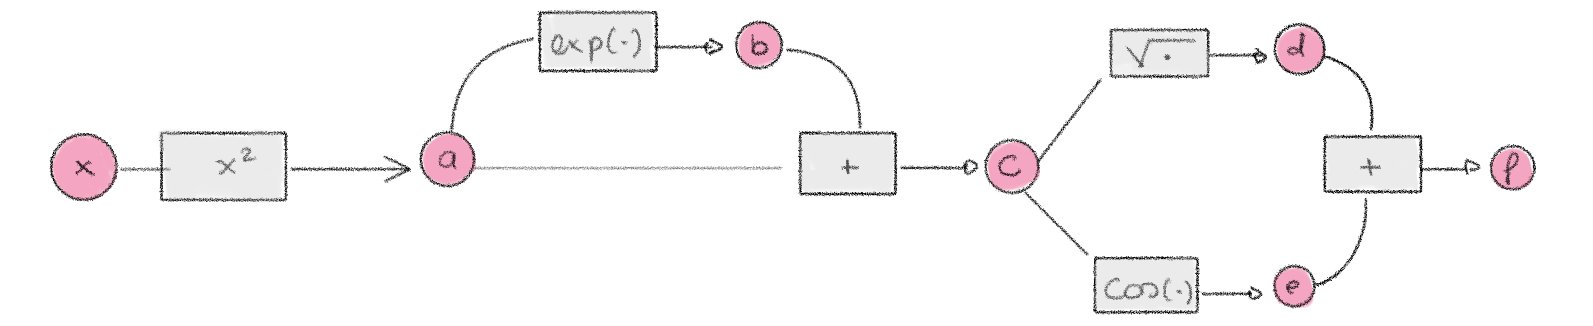
\includegraphics[width=\linewidth]{nn_backpropagation}
    \end{center}
    By looking at the computation graph, we can compute
    $\frac{\partial{f}}{\partial{x}}$ by working backward from the end of the
    graph and obtain the derivative of each variable, making the use of the
    derivatives of the children of that variable
    $$\begin{aligned}
        \frac{\partial{f}}{\partial{d}}=\frac{\partial{f}}{\partial{e}}=1 \\
        \frac{\partial{f}}{\partial{c}}=\frac{\partial{f}}{\partial{d}}\frac{\partial{d}}{\partial{c}}+\frac{\partial{f}}{\partial{e}}\frac{\partial{e}}{\partial{c}}
        \\ 
        \frac{\partial{f}}{\partial{b}}=\frac{\partial{f}}{\partial{c}}\frac{\partial{c}}{\partial{b}}
        \\
        \frac{\partial{f}}{\partial{a}}=\frac{\partial{f}}{\partial{b}}\frac{\partial{b}}{\partial{a}}+\frac{\partial{f}}{\partial{c}}\frac{\partial{c}}{\partial{a}}
        \\ 
        \frac{\partial{f}}{\partial{x}}=\frac{\partial{f}}{\partial{a}}\frac{\partial{a}}{\partial{x}}
    \end{aligned}$$
    We observe that the computation required for calculating the derivative is
    of similar complexity as the computation of the function itself (forward
    pass).
\end{example}
Automatic differentiation is a formalization of last Example. Let
$x_1,\ldots,x_d$ be the input variables to the function,
$x_{d+1},\ldots,x_{D-1}$ be the intermediate variables, and $x_D$ the output
variable. Then the computation graph can be expressed as follows:
\begin{equation}\label{eq:forward_pass}
    \text{For }i=d+1,\ldots,D:\quad x_i=g_i(x_{Pa}(x_i))
\end{equation}
where the $g_i(\cdot)$ are elementary functions and $x_{Pa}(x_i)$ are the
parent nodes of the variable $x_i$ in the graph.

Recall that by definition $f=x_D$ and hence
$$\frac{\partial{f}}{\partial{x_D}}=1$$
For other variables $x_i$, we apply the chain rule 
\begin{equation}\label{eq:backward_pass}
    \frac{\partial{f}}{\partial{x_i}}=\displaystyle\sum_{x_j:x_i\in
    Pa(x_j)}\frac{\partial{f}}{\partial{x_j}}\frac{\partial{x_j}}{\partial{x_i}}=\displaystyle\sum_{x_j:x_i\in
    Pa(x_j)}\frac{\partial{f}}{\partial{x_j}}\frac{\partial{g_j}}{\partial{x_i}}
\end{equation}
where $Pa(x_j)$ is the set of parent nodes of $x_j$ in the computation graph.
Equation \ref{eq:forward_pass} is the \underline{forward pass}, whereas
\ref{eq:backward_pass} is the \underline{backward pass}.

The automatic differentiation approach works whenever we have a function that
can be expressed as a computation graph, where the elementary functions are
differentiable. 
\cleardoublepage
\section{Continuous Optimization}
Training a machine learning essentially involves identifying a good set of
parameters. What constitutes ``good'' is defined by the objective function.
Optimization algorithms are employed to locate the best possible value of this
function. Typically, the aim is to minimize the objective function, implying
that the best value is the minimum one.

\begin{figure}[!h]
   \centering
   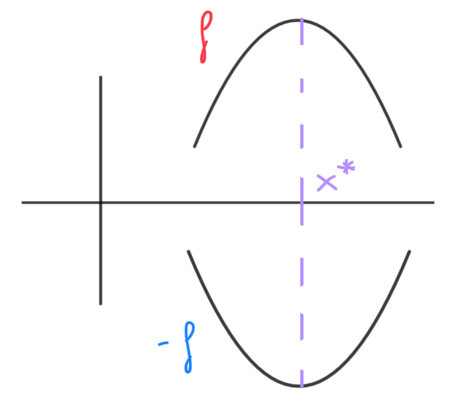
\includegraphics[width=0.25\linewidth]{argmin_argmax}
   \caption{$\underset{x\in \mathbb{R}^N}\argmax\
   f(x)=\underset{x\in\mathbb{R}^N}\argmin\ {f(x)}$}
\end{figure}

We will assume in this chapter that our objective function is
differentiable, hence we have access to a gradient to help us find the
optimal value. Intuitively, finding the best value is like finding the valleys
of the objective function, and the gradients point us uphill. The idea is to
move downhill (opposite to the gradient) and hope to find the deepest point.
\subsection{Conditions for the existence of the minimum} 
\begin{definition}
    A $f:\mathbb{R}^n\to \mathbb{R}$ is continuous and differentiable if
    the partial derivates $\frac{\partial{f}}{\partial{x_i}},i=1,\ldots,N$
    exist and are continuous. 
\end{definition}
\begin{definition}
    $x^*\in \mathbb{R}^N$ is a (strict) \textbf{local minimum} for $f$ if 
    $$f(x^*)(<)\leq f(x)\quad \forall x: \lVert x-x^*\rVert<\epsilon$$
\end{definition}
\begin{definition}
    $x^*\in \mathbb{R}^N$ is a (strict) \textbf{global minimum} for $f$ if 
    $$f(x^*)(<)\leq f(x)\quad \forall x\in \mathbb{R}^N$$
\end{definition}
\begin{center}
    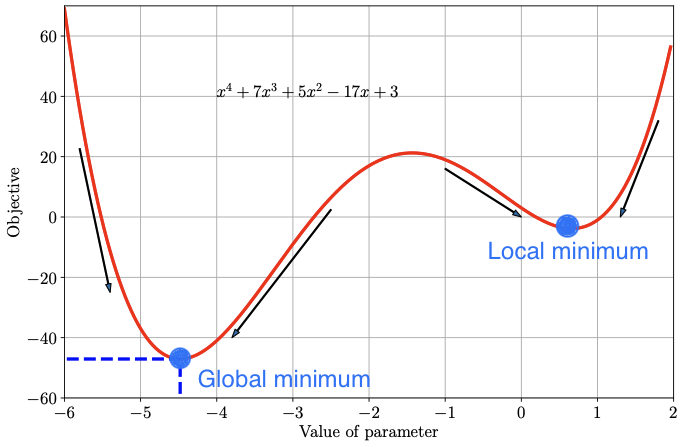
\includegraphics[width=0.75\linewidth]{local_global_minimum}
\end{center}
\subsubsection{Optimality Conditions}
\begin{definition}[First order conditions]
    If $x^*$ is a minimum point of $f$, then $\nabla f(x^*)=0$. Furthermore,
    if $\nabla f(x^*)=0$ for $x^*\in \mathbb{R}^N$, then $x^*$ can be either a
    (local) minimum, a (local) maximum or a saddle point of $f(x)$.
\end{definition}
Consequently, we want to find a point $x^*\in \mathbb{R}^N$ such that $\nabla
f(x^*)=0$. Those points are stationary points for $f$.
\begin{center}
    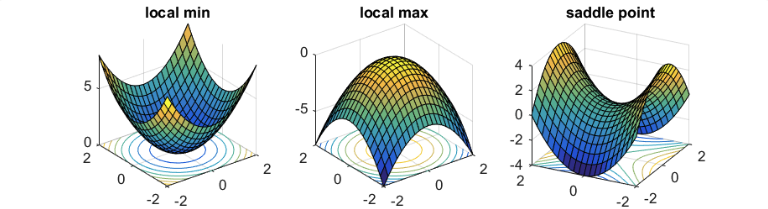
\includegraphics[width=\linewidth]{min_max_saddle}
\end{center}
\begin{definition}[Second order conditions]
    if $f$ is twice differentiable and if $\nabla f(x^*)=0$ and t
    
\end{definition}
\subsection{Algorithm to compute the minimum}
\end{document}
